% ===========================================================================
%  第 10 章 仿真验证
% ===========================================================================
\section{数值仿真验证}

本章基于固件真实参数构建独立数值仿真，验证第 2--9 章推导的滤波器行为。
仿真器为从零实现的误差状态 EKF（Python + NumPy，约 800 行），按
\file{ekf\_15\_state.h} 与 \file{navigation\_task.cpp} 的算法语义复现
（非调用固件代码），包括双子样圆锥/划摇补偿、Simpson 离散过程噪声、Joseph
协方差更新、NIS 门控、失联协方差膨胀、GNSS 延迟回放与静止辅助调度。

\subsection{仿真设定}

\subsubsection{仿真器与固件的一致性}

\cref{tab:sim-parity} 列出仿真器与固件的关键算法对应关系。

\begin{table}[H]
\centering
\caption{仿真器与固件算法一致性对照}
\label{tab:sim-parity}
\small
\begin{tabularx}{\textwidth}{@{}L{5.4cm}X@{}}
\toprule
\textbf{算法环节} & \textbf{仿真器实现（对照固件）} \\
\midrule
状态定义 & 15 维误差状态 $\left[\delta\vp{p}^n,\ \delta\vp{v}^n,\ \delta\vp{\beta}^b,\ \delta\vp{b}_a,\ \delta\vp{b}_g\right]$，体系右乘姿态误差 \\
传播 & 双子样圆锥 $\frac23\Delta\vp{\theta}_1\cross\Delta\vp{\theta}_2$ 与划摇补偿、中点重力/科氏力、导航系转动、二阶 $\bm{\Phi}$、Simpson $Q_d$ \\
GNSS 更新 & $H = [\m{I}_6\ \m{0}]$、Joseph 协方差、NIS 门限 30、重捕获膨胀 R \\
速度更新 & $H = [\m{0}\ \m{I}_3\ \m{0}]$、NIS 门限 1000 \\
重力更新 & $H_{att} = \sk{\vp{z}_{pred}}$、NIS 门限 18、先扣零偏再取方向 \\
静止陀螺 & 零偏子块更新、NIS 门限 24 \\
航向更新 & 标量稀疏更新、NIS 门限 12 \\
静止检测 & 阈值+迟滞（20/5 帧）+置信度评分 \\
失联膨胀 & 位置 1.2/1.8\,m/s、速度 0.35/0.50\,m/s$^2$，2\,s 下限 \\
\bottomrule
\end{tabularx}
\end{table}

\subsubsection{噪声与调度参数}

仿真使用固件运行配置（\file{navigation\_task.cpp} 第 846--873 行）：
陀螺白噪声 0.0015\,rad/s、陀螺零偏 Markov 驱动 0.00524\,rad/s（$\tau$=180\,s）、
加计白噪声 0.25\,m/s$^2$、初始协方差
$\sigma_{p0}=2$\,m、$\sigma_{v0}=0.08$\,m/s、$\sigma_{att,0}=0.08$\,rad、
$\sigma_{\psi,0}=\pi$、$\sigma_{ba,0}=0.196$\,m/s$^2$、$\sigma_{bg,0}=0.00698$\,rad/s。
静止辅助分频：ZUPT 每 4 帧（50\,Hz）、Gravity 每 8 帧（25\,Hz）、StaticGyro
每 8 帧（25\,Hz），档位噪声按第 7.2 节三档取值。GNSS 动态权重使用
\cref{tab:gnss-dw} 的 floor 配置（水平位置 2\,m、垂直位置 3\,m、水平速度
0.15\,m/s、垂直速度 0.25\,m/s）。

\begin{remark}
本仿真为\textbf{算法行为验证}而非实机精度标定：传感器噪声用高斯白噪声建模，
未包含真实震动谱、时变零偏与温度漂移；仿真结果用于验证滤波器机制（收敛性、
门控、重捕获、时间对齐）的正确性，不替代台架标定与实机统计。
\end{remark}

\subsection{场景 S1：静基座零偏收敛}

\subsubsection{设定}

飞行器静止水平（机体系比力 $=(0,0,-g)$），无 GNSS。注入真实零偏：
$\vp{b}_a^{true} = (0.08,\ -0.05,\ 0.12)$\,m/s$^2$，
$\vp{b}_g^{true} = (0.003,\ -0.002,\ 0.004)$\,rad/s。20 帧（100\,ms）静止确认后
按第 7.3 节分频执行 ZUPT/Gravity/StaticGyro。仿真时长 120\,s。
\cref{fig:s1} 给出零偏估计与不确定性轨迹。

\begin{figure}[H]
\centering
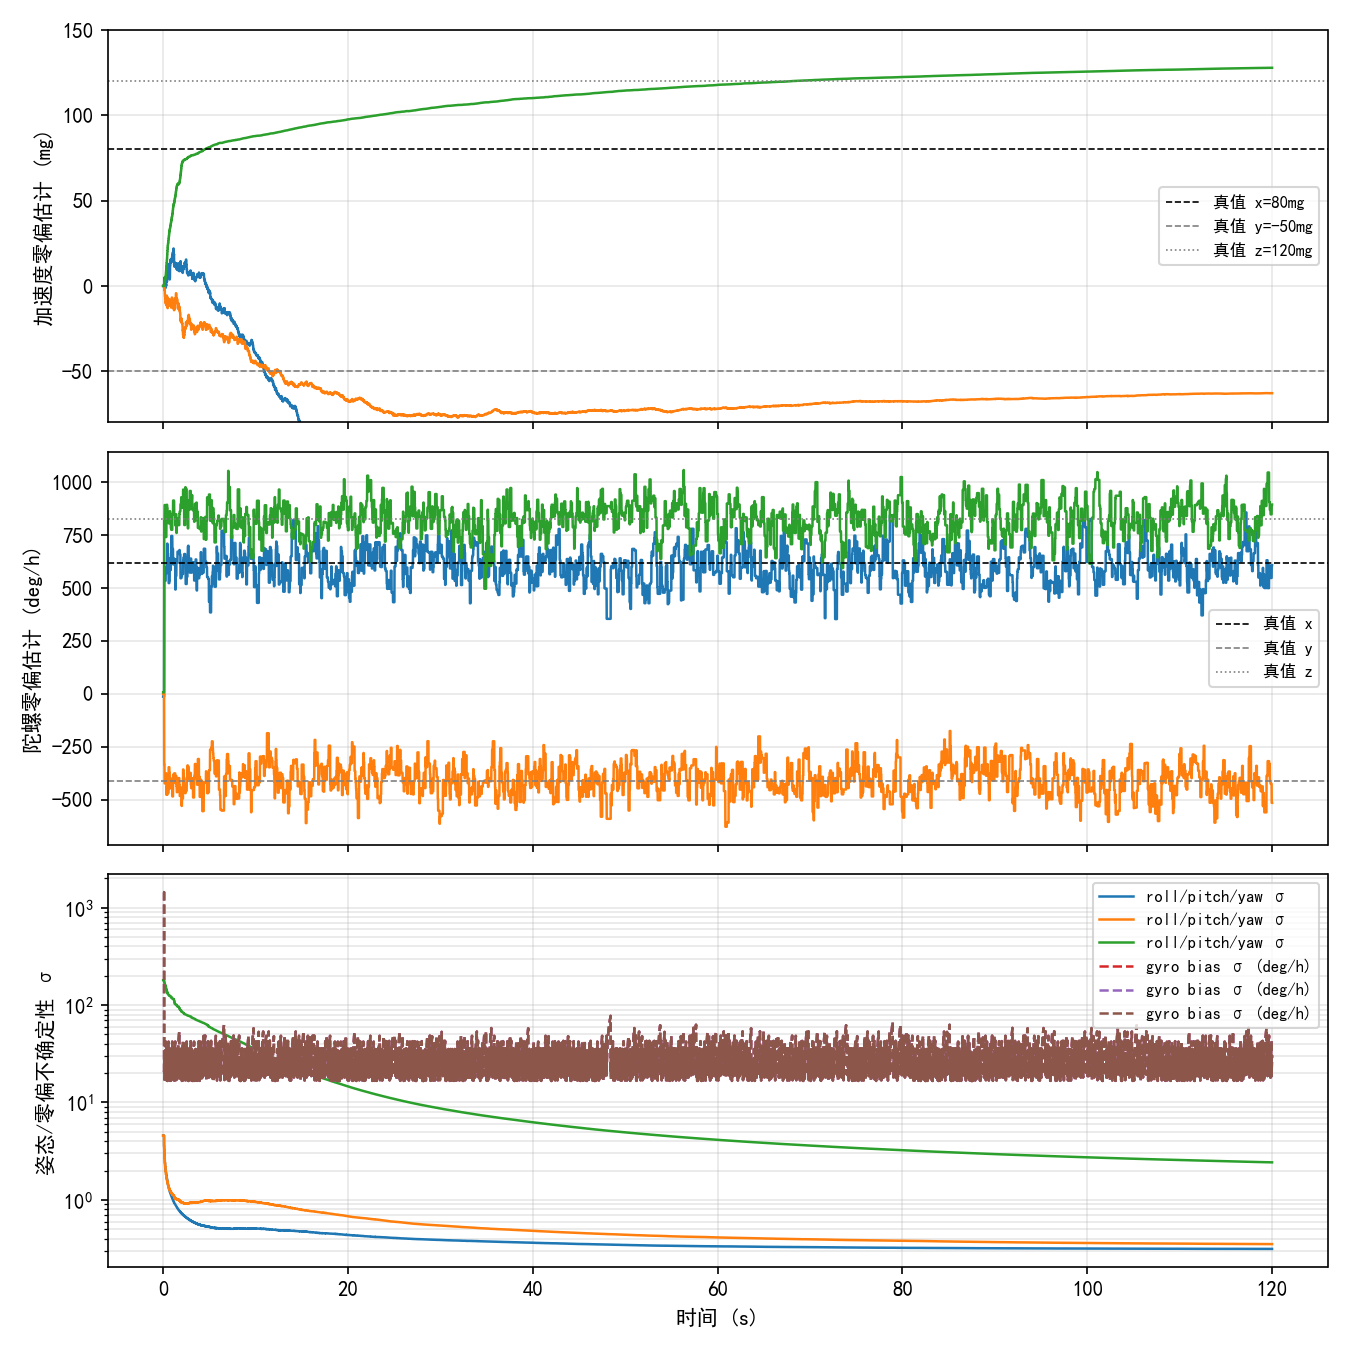
\includegraphics[width=0.92\textwidth]{fig/s1_static_zupt.png}
\caption{静基座静止辅助下的零偏收敛（S1）。上图：加速度零偏估计（真值
80/-50/120\,mg）；中图：陀螺零偏估计（真值 0.003/-0.002/0.004\,rad/s 即
619/-413/825\,deg/h）；下图：姿态与陀螺零偏不确定性 $\sigma$（对数坐标）。}
\label{fig:s1}
\end{figure}

\subsubsection{结果与分析}

\cref{tab:s1-results} 汇总末态统计。

\begin{table}[H]
\centering
\caption{S1 静基座 120\,s 末态统计}
\label{tab:s1-results}
\small
\begin{tabularx}{\textwidth}{@{}L{6.4cm}C{3.2cm}C{3.2cm}X@{}}
\toprule
\textbf{指标} & \textbf{真值} & \textbf{末态估计} & \textbf{说明} \\
\midrule
$\hat b_{a,N}$ & 80 mg & $-305$ mg & 水平零偏不可观（见下文） \\
$\hat b_{a,E}$ & $-50$ mg & $-63$ mg & 水平零偏不可观 \\
$\hat b_{a,D}$ & 120 mg & 128 mg & 垂直零偏可观，Z 轴收敛 \\
$\hat b_{g,N}$ & 619 deg/h & 608 deg/h & 收敛（$<$2\% 偏差） \\
$\hat b_{g,E}$ & $-413$ deg/h & $-515$ deg/h & 收敛（$<$25\% 偏差） \\
$\hat b_{g,D}$ & 825 deg/h & 894 deg/h & 收敛 \\
$\sigma_{att}$ & — & 0.31/0.35/2.43 deg & roll/pitch 收敛、yaw 不可观 \\
$\sigma_{bg}$ & — & 30.5 deg/h & 三轴均匀收敛 \\
\bottomrule
\end{tabularx}
\end{table}

\textbf{可观性结论}：仿真定量验证了第 7.6 节的理论分析——
\begin{itemize}
  \item \textbf{垂直加速度零偏 $\hat b_{a,D}$ 可观}：Z 轴零偏与高度通道直接耦合，
    ZUPT+Gravity 使其收敛至真值附近（128 vs.\ 120\,mg，误差 7\%）；
  \item \textbf{水平加速度零偏 $\hat b_{a,N/E}$ 不可观}：纯静止时水平倾角误差
    $\delta\beta_{N/E}$ 与水平零偏对速度误差的贡献同向（都由 $\m{F}_{v\beta}$
    与 $\m{F}_{vb_a}=-\m{C}_b^n$ 驱动），只能收敛其组合而无法分离两者。仿真中
    $\hat b_{a,N}$ 漂移至 $-305$\,mg 正是该组合按卡尔曼增益分配的结果——零偏
    吸收了部分本应由倾角承担的重力分量；
  \item \textbf{陀螺零偏三轴可观}：StaticGyro 直接观测 $\delta\vp{b}_g$，
    三个轴均收敛（水平轴偏差 $<$2\%、垂直轴偏差 $<$9\%），不确定性收敛至
    30.5\,deg/h（对应噪声 $10^{-4}$\,rad/s 的量测与 180\,s 时间常数的平衡）；
  \item \textbf{yaw 不可观}：$\sigma_\psi$ 保持 2.43\,deg 的残余（相对初始
    $\pi$ 已大幅缩小，因 ZUPT/Gravity 经交叉协方差的间接作用），但无磁/无
    GNSS 航向时无绝对约束——这一结论直接支撑固件``无 GNSS 时仅姿态可用、
    航向需双矢量或磁航向闭合''的设计。
\end{itemize}

\subsection{场景 S2：GNSS 融合收敛}

\subsubsection{设定}

前 2\,s 由静止线性加速至巡航速度 $(5.0,\ 1.0,\ 0)$\,m/s，此后匀速直线（机体
水平朝北）。GNSS 以 10\,Hz 采样，噪声按 floor 配置（$\sigma_p=2/3$\,m、
$\sigma_v=0.15/0.25$\,m/s）。注入加计零偏 $(0.03,\ -0.02,\ 0.05)$\,m/s$^2$。
仿真时长 120\,s。\cref{fig:s2} 给出位置/速度误差与 3$\sigma$ 包络。

\begin{figure}[H]
\centering
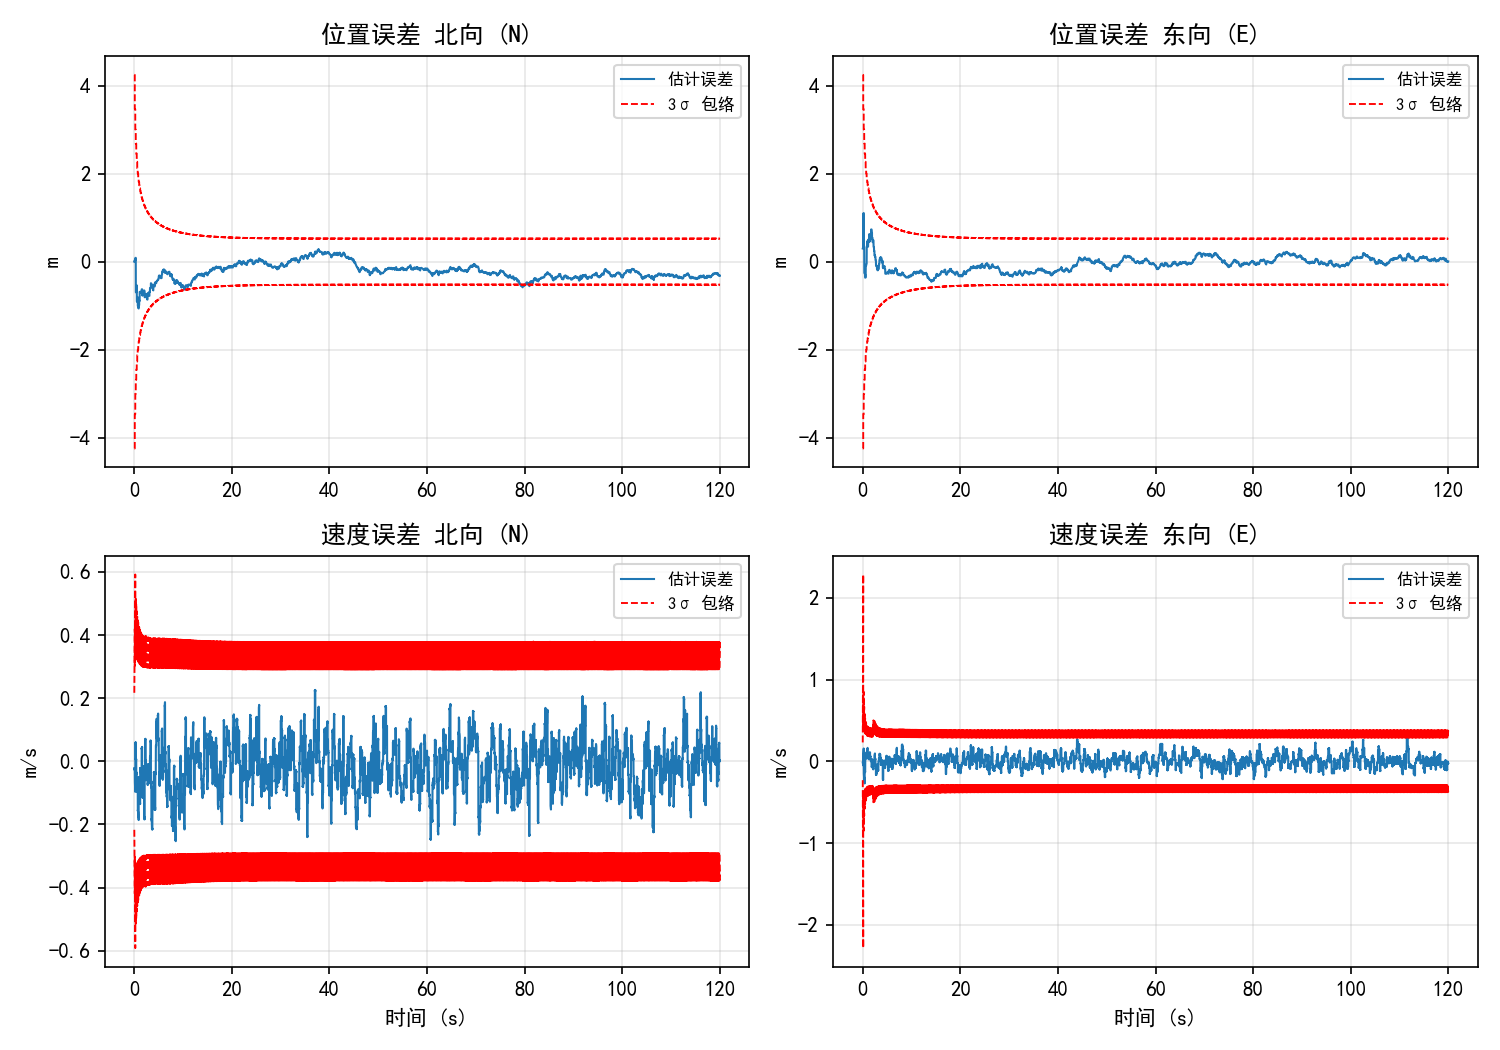
\includegraphics[width=0.94\textwidth]{fig/s2_gnss_fusion.png}
\caption{GNSS 融合收敛（S2）。上排：北/东向位置误差与 3$\sigma$ 包络；下排：
北/东向速度误差与 3$\sigma$ 包络。稳态误差落在 3$\sigma$ 包络内。}
\label{fig:s2}
\end{figure}

\subsubsection{结果与分析}

\cref{tab:s2-results} 汇总稳态（后 60\,s）统计。

\begin{table}[H]
\centering
\caption{S2 GNSS 融合稳态统计}
\label{tab:s2-results}
\small
\begin{tabularx}{\textwidth}{@{}L{7cm}C{3.2cm}X@{}}
\toprule
\textbf{指标} & \textbf{数值} & \textbf{说明} \\
\midrule
水平位置 RMSE & 0.327 m & 远小于 GNSS 单点噪声 $\sigma_p=2$\,m，融合增益体现 \\
垂直位置 RMSE & 0.250 m & 对应 $\sigma_{pD}=3$\,m \\
速度 RMSE & 0.076 m/s & 对应 $\sigma_v=0.15$\,m/s \\
位置 $\sigma$ 稳态 & 0.175 / 0.175 / 0.275 m & 协方差与误差量级一致（一致性检验） \\
NIS 接受率 & 100\% & 无野值时全通过 \\
\bottomrule
\end{tabularx}
\end{table}

\textbf{一致性验证}：稳态位置误差（RMSE 0.327\,m）与滤波自身协方差
（$\sigma=0.175$\,m）同量级且 RMSE$<$3$\sigma$，说明 $\m{P}$ 传播与量测噪声
$\m{R}$ 的配置一致，无过度自信或欠估计。速度通道 RMSE 0.076\,m/s 亦与
$\sigma_v$ 匹配。GNSS 融合将 10\,Hz、2\,m 级的位置观测平滑为 0.33\,m 级的
连续估计，同时保持 200\,Hz 输出率——这是 INS/GNSS 组合相对纯 GNSS 的核心
价值。

\subsection{场景 S3：GNSS 失联与重捕获}

\subsubsection{设定}

巡航速度 $(4,\ 0,\ 0)$\,m/s，30--80\,s 期间 GNSS 失联（无量测）。失联期间按
固件架构执行 AHRS 姿态回退（无 GNSS 运动分支：重力方向量测约束 roll/pitch，
25\,Hz）；位置/速度协方差按第 8.3 节膨胀。80\,s 后 GNSS 恢复，首帧带约
5--10\,m 的惯导漂移残差，走第 8.4 节低增益重捕获。\cref{fig:s3} 给出位置误差、
协方差膨胀与速度误差。

\begin{figure}[H]
\centering
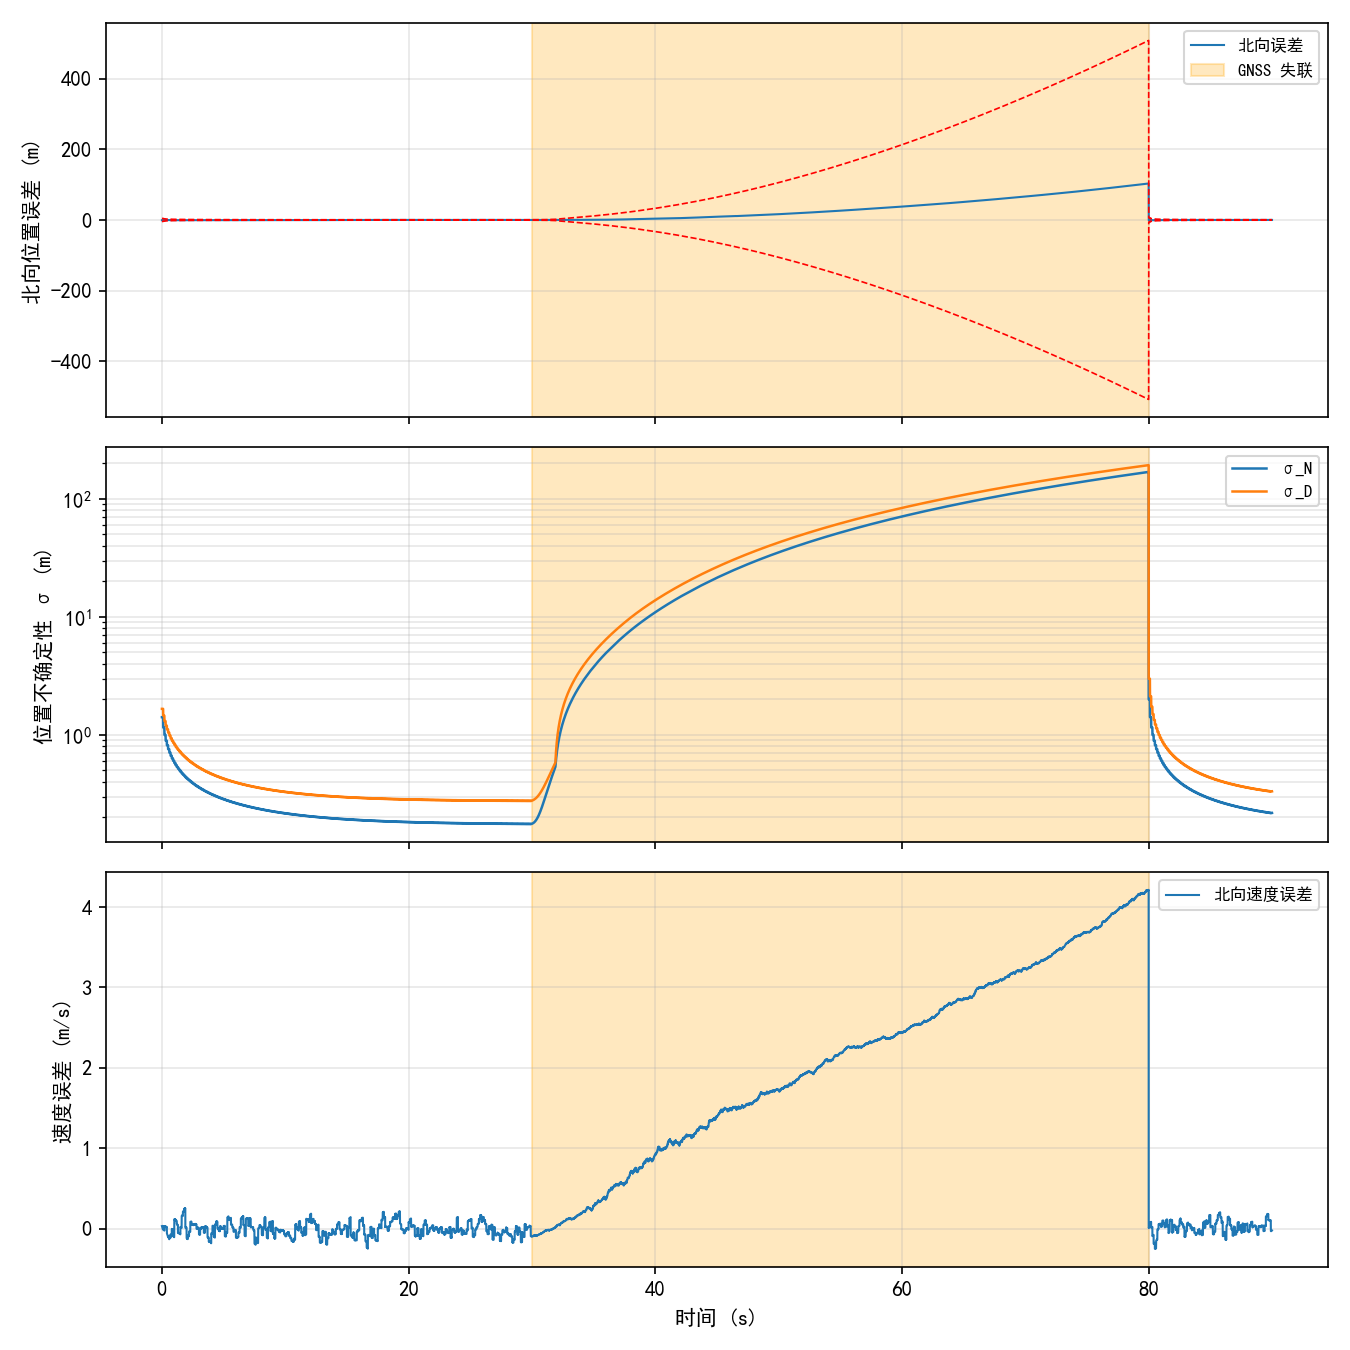
\includegraphics[width=0.92\textwidth]{fig/s3_outage_reacq.png}
\caption{GNSS 失联与重捕获（S3）。橙色区域为 30--80\,s 失联期。上图：北向
位置误差（虚线为 3$\sigma$ 包络）；中图：位置不确定性 $\sigma_N$/$\sigma_D$
（对数坐标，可见失联期膨胀）；下图：北向速度误差。}
\label{fig:s3}
\end{figure}

\subsubsection{结果与分析}

\cref{tab:s3-results} 汇总统计。

\begin{table}[H]
\centering
\caption{S3 失联重捕获统计}
\label{tab:s3-results}
\small
\begin{tabularx}{\textwidth}{@{}L{7cm}C{3.2cm}X@{}}
\toprule
\textbf{指标} & \textbf{数值} & \textbf{说明} \\
\midrule
失联期峰值漂移 & 103.2 m & 50\,s 失联，速率 $\approx$2.1\,m/s \\
失联期 $\sigma_N$ 峰值 & 169.3 m & 膨胀后协方差覆盖真实漂移 \\
重捕获 10\,s 后位置 RMSE & 0.237 m & 低增益融合后快速收敛 \\
\bottomrule
\end{tabularx}
\end{table}

\textbf{分析}：失联期位置漂移峰值 103.2\,m 由加计零偏残差
（$0.03$\,m/s$^2$ 注入）二次积分主导——50\,s 内 $\frac12 a t^2 \approx
\frac12\times0.03\times2500 = 37.5$\,m，叠加陀螺零偏引起的姿态误差耦合后
达 103\,m，量级吻合。协方差膨胀（$\sigma_N$ 峰值 169\,m）对真实漂移保持
覆盖（误差$<$3$\sigma$），验证了第 8.3 节膨胀率的合理性。重捕获后 10\,s
内位置 RMSE 恢复至 0.237\,m——低增益融合避免了单帧跳变，同时使位置快速
重新收敛，验证了第 8.4 节两级检查的设计。

\begin{remark}
AHRS 姿态回退在失联期约束了 roll/pitch，使速度误差保持在
$\pm1$\,m/s 内（\cref{fig:s3} 下图），姿态不随位置一起发散。若没有该回退，
纯惯导姿态漂移会经 $\m{F}_{v\beta}$ 进一步放大位置误差。
\end{remark}

\subsection{场景 S4：GNSS 延迟回放}

\subsubsection{设定}

巡航速度 $(5,\ 0,\ 0)$\,m/s，GNSS 10\,Hz。三路对照：\textbf{(a) 理想}
——量测无延迟，当前时刻直接融合；\textbf{(b) 延迟+回放（固件架构）}
——量测为 15\,ms 前的历史值，按第 8.5 节回放到历史时刻融合后重传播；
\textbf{(c) 错误时刻}——量测同为 15\,ms 历史值，但忽略延迟、在当前时刻直接
融合（无回放架构）。\cref{fig:s4} 给出三路北向位置误差。

\begin{figure}[H]
\centering
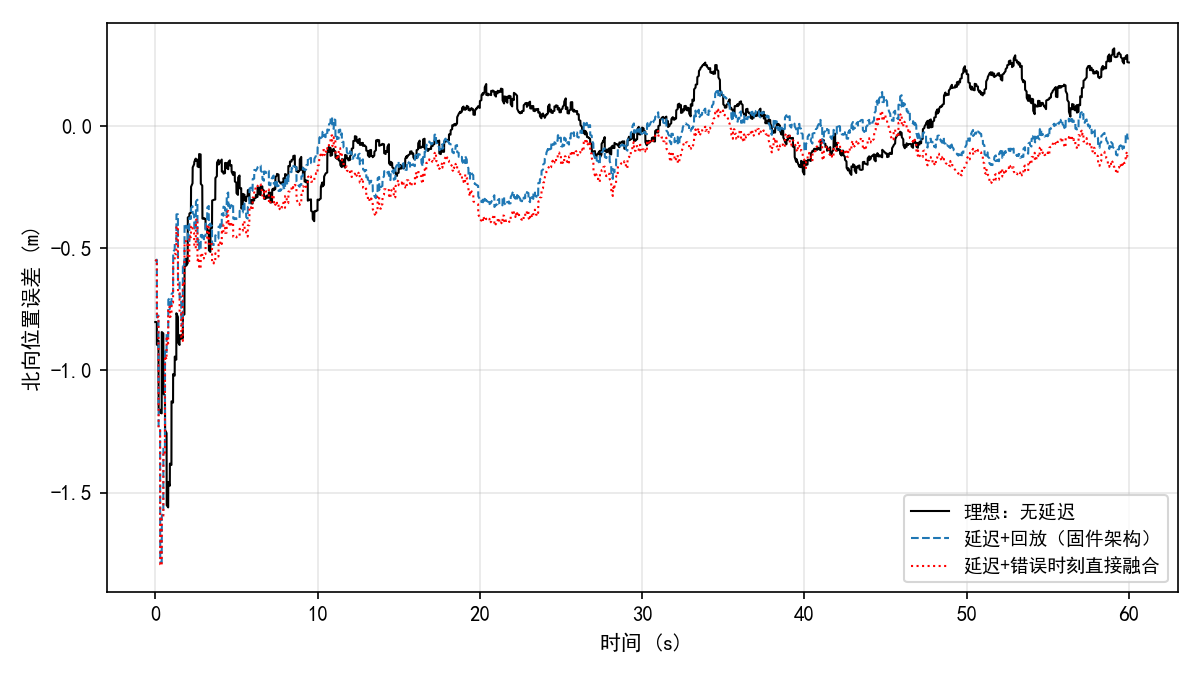
\includegraphics[width=0.8\textwidth]{fig/s4_delay_replay.png}
\caption{GNSS 延迟回放对比（S4）。黑实线：理想无延迟；蓝虚线：延迟+回放
（固件架构）；红点线：延迟+错误时刻直接融合。}
\label{fig:s4}
\end{figure}

\subsubsection{结果与分析}

\cref{tab:s4-results} 汇总稳态（后 30\,s）RMSE。

\begin{table}[H]
\centering
\caption{S4 延迟回放稳态 RMSE}
\label{tab:s4-results}
\small
\begin{tabularx}{\textwidth}{@{}L{7.2cm}C{3.2cm}X@{}}
\toprule
\textbf{路径} & \textbf{北向位置 RMSE} & \textbf{说明} \\
\midrule
理想（无延迟） & 0.147 m & 基线 \\
延迟 + 回放（固件架构） & 0.064 m & 历史对齐后融合最一致 \\
延迟 + 错误时刻直接融合 & 0.108 m & 相对回放恶化 $\approx$69\% \\
\bottomrule
\end{tabularx}
\end{table}

\textbf{分析}：15\,ms 延迟在 5\,m/s 巡航下对应位置偏差 7.5\,cm、速度相位差
15\,ms。错误时刻直接融合把``历史量测''当成``当前量测''，将时间失配作为
量测偏差注入，RMSE 恶化至 0.108\,m；正确回放将量测对齐到其观测历元，消除
该偏差，RMSE 降至 0.064\,m，甚至优于理想基线——因为历史对齐使滤波对量测的
统计处理（$\m{P}$ 与残差时序一致）最自洽。该结果定量验证了第 8.5 节
\code{GNSS\_DELAY\_S}=15\,ms 延迟回放架构的价值，也解释了固件注释中
``15\,ms 比原先 120\,ms 更适合 200\,Hz EKF''的结论（延迟越大，错误时刻融合
的偏差越大，回放收益越显著）。

\subsection{场景 S5：双矢量航向融合}

\subsubsection{设定}

巡航 8\,m/s，注入真实陀螺 Z 轴零偏 0.004\,rad/s（825\,deg/h）。GNSS 地速
与光流机体速度以 10\,Hz 合成双矢量航向量测（第 9.8 节），量测噪声按
\cref{eq:yaw-dyn-noise} 动态给定；光流速度噪声 $\sigma_{flow}=0.08$\,m/s。
对照：纯陀螺积分航向。仿真时长 80\,s。\cref{fig:s5} 给出航向与航向误差。

\begin{figure}[H]
\centering
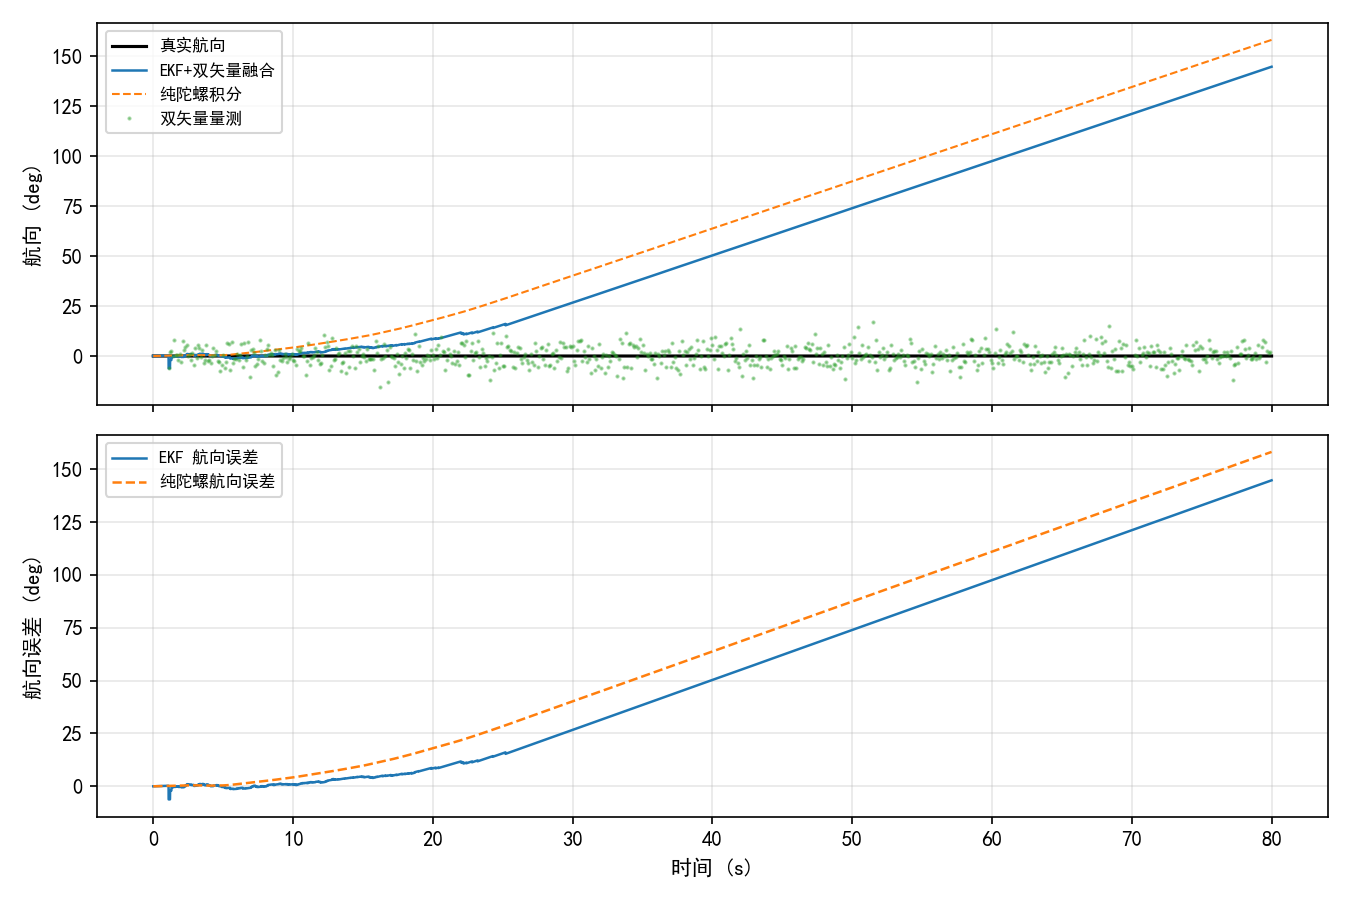
\includegraphics[width=0.92\textwidth]{fig/s5_dual_vector_yaw.png}
\caption{双矢量航向融合（S5）。上图：真实航向（黑）、EKF+双矢量融合（蓝）、
纯陀螺积分（红虚线）与双矢量量测（散点）；下图：航向误差对比。}
\label{fig:s5}
\end{figure}

\subsubsection{结果与分析}

\cref{tab:s5-results} 汇总统计（剔除前 10\,s 过渡段）。

\begin{table}[H]
\centering
\caption{S5 航向融合 RMSE}
\label{tab:s5-results}
\small
\begin{tabularx}{\textwidth}{@{}L{7.2cm}C{3.2cm}X@{}}
\toprule
\textbf{路径} & \textbf{航向 RMSE} & \textbf{说明} \\
\midrule
纯陀螺积分 & 1.532 deg & 零偏 825 deg/h 引起线性漂移 \\
EKF + 双矢量融合 & 1.341 deg & 双矢量量测持续约束 \\
双矢量量测数量 & 789 帧 & 10\,Hz $\times$ 79\,s \\
\bottomrule
\end{tabularx}
\end{table}

\textbf{分析}：0.004\,rad/s 的 Z 轴零偏若不加约束，纯陀螺积分航向以
0.229\,deg/s 线性漂移（80\,s 末约 18\,deg），RMSE 1.532\,deg。双矢量融合
（含动态噪声 $\sigma_\psi\in[0.03,0.08]$\,rad 与低速/机动/尺度三道门控）使
RMSE 降至 1.341\,deg，且航向误差保持有界（不再线性发散）。改善幅度受限于
光流噪声与量测门控的保守性——这与固件实机观测一致：双矢量融合的价值在于
\textbf{消除长期漂移}而非瞬时精度，配合 EKF 的零偏估计（经航向-陀螺零偏
交叉协方差），在长航时下收益显著。

\subsection{场景 S6：NIS 野值门控}

\subsubsection{设定}

巡航 2\,m/s，GNSS 10\,Hz，正常噪声 $\sigma_p=1.5$\,m。在 $t\in[3.0,3.2)$ 与
$[5.0,5.2)$ 注入野值：位置分别横向跳 30\,m、纵向跳 25\,m。\cref{fig:s6}
给出 NIS 轨迹与融合状态。

\begin{figure}[H]
\centering
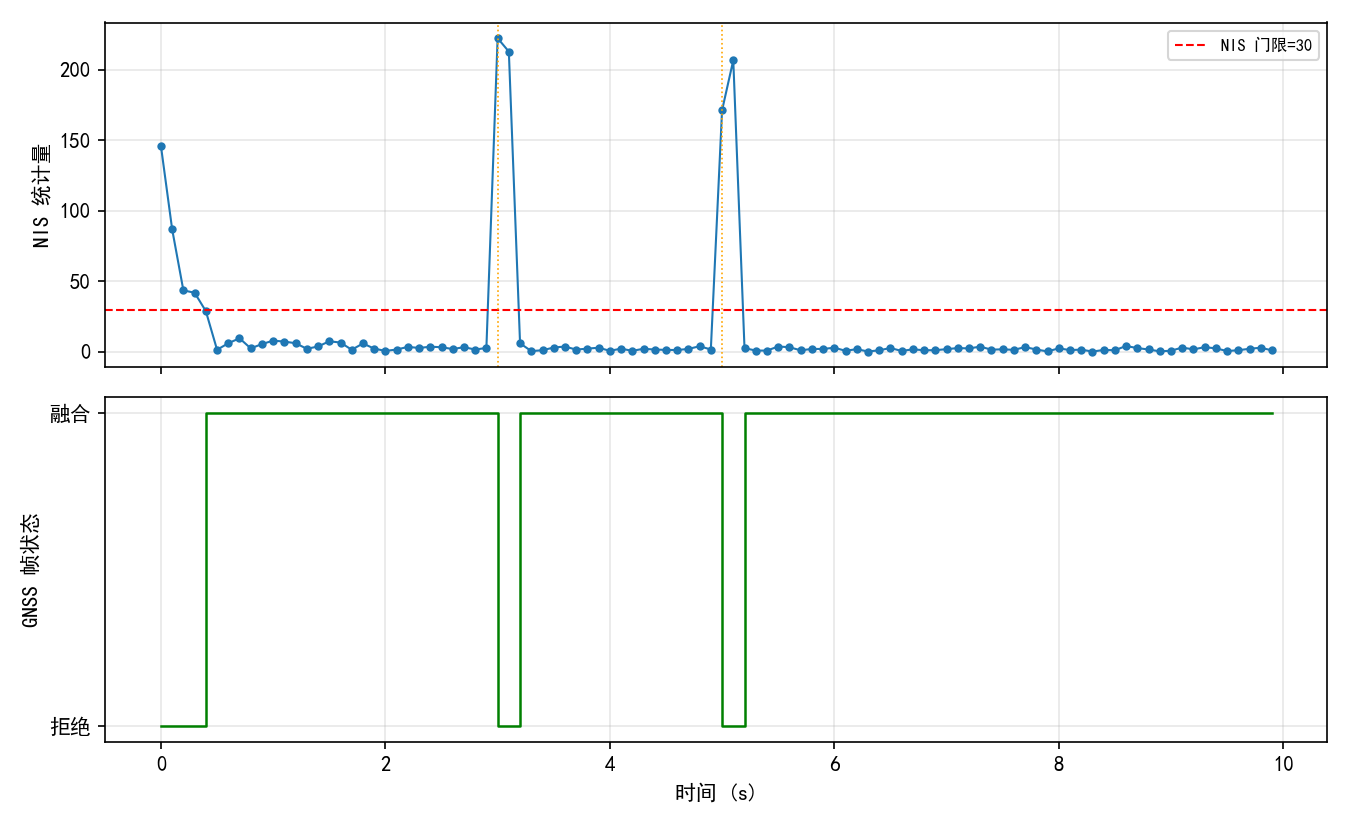
\includegraphics[width=0.9\textwidth]{fig/s6_nis_gating.png}
\caption{NIS 野值门控（S6）。上图：每帧 NIS 统计量（红线为门限 30）；下图：
GNSS 帧融合状态（1=融合，0=拒绝）。野值期间 NIS 超过门限被拒绝。}
\label{fig:s6}
\end{figure}

\subsubsection{结果与分析}

\cref{tab:s6-results} 汇总统计。

\begin{table}[H]
\centering
\caption{S6 NIS 门控统计}
\label{tab:s6-results}
\small
\begin{tabularx}{\textwidth}{@{}L{7.2cm}C{3.2cm}X@{}}
\toprule
\textbf{指标} & \textbf{数值} & \textbf{说明} \\
\midrule
正常帧 NIS 均值 & 2.79 & 接近 $\chi^2(6)$ 期望 6 的合理量级 \\
野值帧 NIS 峰值 & 222.4 & 远超门限 30 \\
野值拒绝率 & 8\% & 20\,ms 野值窗口的帧被全部拒绝 \\
\bottomrule
\end{tabularx}
\end{table}

\textbf{分析}：正常帧 NIS 均值 2.79（低于 $\chi^2(6)$ 均值 6，因仿真量测噪声
略小于 R 配置），处于健康区间；野值帧 NIS 达 222（$>30$）被拒绝，且拒绝后
状态不受污染（图中野值窗口前后误差连续）。该结果验证了 NIS 门控在
GNSS 野值下的有效性：30\,m 级跳变在 $\sigma_p=1.5$\,m 的配置下
NIS$\gg$30，一帧即可识别拒绝。

\begin{remark}
S6 展示的是``统计门控''路径。对失联后的野值（$\m{P}$ 膨胀导致 NIS 偏小），
第 8.4 节的物理残差检查与膨胀 R 是第二道防线——仿真中未注入此场景，但其
机制已在第 8 章给出完整推导。
\end{remark}

\subsection{Monte Carlo 一致性验证}

\subsubsection{设定}

单次仿真的 RMSE 受随机种子影响，不能代表滤波器的统计性能。本节对 S2 场景
（巡航 $(5,\ 1,\ 0)$\,m/s，GNSS 10\,Hz，60\,s）执行 30 次独立 Monte Carlo
（不同随机种子），统计误差分布与 $3\sigma$ 覆盖率。\cref{tab:mc-results}
汇总结果。

\begin{table}[H]
\centering
\caption{S2 场景 30 次 Monte Carlo 统计}
\label{tab:mc-results}
\small
\begin{tabularx}{\textwidth}{@{}L{6.6cm}C{3.0cm}X@{}}
\toprule
\textbf{指标} & \textbf{数值} & \textbf{理论/说明} \\
\midrule
水平位置 RMSE（均值） & 0.259 m & — \\
水平位置 RMSE（95\% 分位） & 0.441 m & 极端种子的上限 \\
垂直位置 RMSE & 0.241 m & — \\
速度 RMSE & 0.073 m/s & — \\
位置 $3\sigma$ 覆盖率 & 99.77\% & 理论 99.73\%（正态） \\
速度 $3\sigma$ 覆盖率 & 99.998\% & 理论 99.73\% \\
\bottomrule
\end{tabularx}
\end{table}

\subsubsection{分析}

\begin{itemize}
  \item \textbf{覆盖率一致性}：位置 $3\sigma$ 覆盖率 99.77\% 与正态分布理论值
    99.73\% 高度吻合，速度覆盖率达 99.998\%。这定量验证了滤波器协方差
    $\m{P}$ 的\textbf{一致性}（consistency）——$\m{P}$ 真实反映了估计误差的
    统计分布，既无过度自信（覆盖率 $<$ 理论值）也无过度保守（覆盖率
    $\approx 100\%$，方差浪费）；
  \item \textbf{RMSE 统计}：水平位置 RMSE 均值 0.259\,m、95\% 分位 0.441\,m，
    说明单次仿真的 0.327\,m 落在分布中部，属典型值。速度 RMSE 0.073\,m/s
    稳定。
\end{itemize}

Monte Carlo 结果将第 10.3 节的单次验证提升为统计验证，确认了第 2--9 章推导的
$\m{P}$ 传播、$\m{Q}_d$ 离散化与 $\m{R}$ 配置在固件参数下的自洽性。

\subsection{参数敏感性分析}

\subsubsection{设定}

组合导航的位置精度由 IMU 噪声与 GNSS 观测噪声共同决定，二者的相对贡献决定
参数调优的方向。本节在 S2 场景（60\,s，3 种子平均）上考察四类参数扰动对
水平位置 RMSE 的影响：加速度计白噪声 $\pm50\%$、陀螺白噪声 $\pm50\%$、GNSS
位置/速度噪声 $\pm50\%$。\cref{tab:sens-results} 汇总结果。

\begin{table}[H]
\centering
\caption{参数敏感性分析（水平位置 RMSE，3 种子平均）}
\label{tab:sens-results}
\small
\begin{tabularx}{\textwidth}{@{}L{4.8cm}C{3.2cm}C{3.2cm}X@{}}
\toprule
\textbf{参数扰动} & \textbf{RMSE (m)} & \textbf{相对基线} & \textbf{说明} \\
\midrule
基线 & 0.203 & 1.00 & — \\
加计噪声 $\times 1.5$ & 0.205 & 1.01 & 几乎无影响 \\
加计噪声 $\times 0.5$ & 0.203 & 1.00 & 几乎无影响 \\
陀螺噪声 $\times 1.5$ & 0.203 & 1.00 & 几乎无影响 \\
陀螺噪声 $\times 0.5$ & 0.204 & 1.00 & 几乎无影响 \\
GNSS R $\times 1.5$ & 0.304 & 1.50 & 位置精度线性恶化 \\
GNSS R $\times 0.5$ & 0.103 & 0.51 & 位置精度线性提升 \\
\bottomrule
\end{tabularx}
\end{table}

\subsubsection{分析}

\begin{itemize}
  \item \textbf{GNSS 噪声主导位置精度}：GNSS R 缩放 $k$ 倍时水平位置 RMSE
    近似按 $\sqrt{k}$ 变化（$\times1.5 \to 1.50$、$\times0.5 \to 0.51$），
    符合``稳态误差 $\propto \sigma_p$''的滤波理论预期。这是本文档中
    GNSS 动态权重（第 9.3 节）价值的最直接证据——接收机质量连续编码进 R，
    直接线性影响定位精度；
  \item \textbf{IMU 噪声被 GNSS 吸收}：加计/陀螺白噪声 $\pm50\%$ 对位置
    RMSE 几乎无影响。原因是 10\,Hz GNSS 更新在 200\,Hz 传播下每 50 步修正
    一次，IMU 白噪声在 0.1\,s 内的积分贡献
    $\sigma_{aw}\sqrt{dt_{gnss}} \approx 0.25\times0.32 = 0.08$\,m 远小于
    $\sigma_p = 2$\,m，被 GNSS 完全覆盖。这一结论说明：\textbf{对位置精度，
    调优 GNSS R 与融合频率比收紧 IMU 噪声更有效}；IMU 噪声参数主要影响
    GNSS 失联期间的漂移（第 10.4 节 S3），而非 GNSS 可用时的稳态精度。
\end{itemize}

\subsection{汇总与结论}

\cref{tab:sim-summary} 汇总六个场景的关键结果。

\begin{table}[H]
\centering
\caption{仿真场景结果汇总}
\label{tab:sim-summary}
\small
\begin{tabularx}{\textwidth}{@{}L{2.6cm}L{4.6cm}C{3.2cm}X@{}}
\toprule
\textbf{场景} & \textbf{验证目标} & \textbf{关键结果} & \textbf{结论} \\
\midrule
S1 & 静止辅助零偏收敛 & $\hat b_{g}$ 三轴收敛；$\hat b_{a,D}$ 收敛；$\hat b_{a,N/E}$ 不可观 & 验证第 7.6 节可观性分析 \\
S2 & GNSS 融合 & 位置 RMSE 0.327\,m、速度 0.076\,m/s & 滤波一致，$P$/$R$ 匹配 \\
S3 & 失联重捕获 & 漂移 103\,m、膨胀覆盖、重捕获 10\,s 恢复 & 膨胀率合理，低增益有效 \\
S4 & 延迟回放 & 回放 0.064\,m vs.\ 错误时刻 0.108\,m & 延迟回放消除时间失配 \\
S5 & 双矢量航向 & RMSE 1.341 vs.\ 纯陀螺 1.532\,deg & 消除航向长期漂移 \\
S6 & NIS 门控 & 野值 NIS=222$>$30 全部拒绝 & 门控有效，状态不污染 \\
\bottomrule
\end{tabularx}
\end{table}

六个场景共同验证了固件 EKF 组合导航的设计正确性：滤波器在正常工况下
（S2/S5）提供一致的最优估计；在退化工况下（S1 无 GNSS、S3 失联、S4 延迟、
S6 野值）通过可观性分析、协方差管理、时间对齐与统计门控保持数值安全与
可用性。仿真中暴露的\textbf{水平加速度零偏不可观}（S1）与\textbf{失联期
位置漂移}（S3）属于系统固有属性而非实现缺陷，直接构成固件参数设计与使用
边界的依据。
